% Copyright 2007 by Mark Wibrow
%
% This file may be distributed and/or modified
%
% 1. under the LaTeX Project Public License and/or
% 2. under the GNU Free Documentation License.
%
% See the file doc/generic/pgf/licenses/LICENSE for more details.


\section{Mathematical Expressions}
\label{pgfmath-syntax}

The easiest way of using \pgfname's mathematical engine is to provide a
mathematical expression given in familiar infix notation, for example,
|1cm+4*2cm/5.5| or |2*3+3*sin(30)|. This expression can be parsed by the
mathematical engine and the result can be placed in a dimension register, a
counter, or a macro.

It should be noted that all calculations must not exceed $\pm16383.99999$ at
\emph{any} point, because the underlying computations rely on \TeX{}
dimensions. This means that many of the underlying computations are necessarily
approximate and, in addition, not very fast. \TeX{} is, after all, a
typesetting language and not ideally suited to relatively advanced mathematical
operations. However, it is possible to change the computations as described in
Section~\ref{pgfmath-reimplement}.

In the present section, the high-level macros for parsing an expression are
explained first, then the syntax for expression is explained.


\subsection{Parsing Expressions}
\label{pgfmath-registers}
\label{pgfmath-parsing}

\subsubsection{Commands}

The \todosp{why 2 labels?}basic command for invoking the parser of \pgfname's
mathematical engine is the following:

\begin{command}{\pgfmathparse\marg{expression}}
    This macro parses \meta{expression} and returns the result without units in
    the macro |\pgfmathresult|.

    \example |\pgfmathparse{2pt+3.5pt}| will set |\pgfmathresult| to the text
    |5.5|.

    In the following, the special properties of this command are explained. The
    exact syntax of mathematical expressions is explained in Sections
    \ref{pgfmath-operators} and~\ref{pgfmath-functions}.
    %
    \begin{itemize}
        \item The result stored in the macro |\pgfmathresult| is a decimal
            \emph{without units}. This is true regardless of whether the
            \meta{expression} contains any unit specification. All numbers with
            units are converted to points first. See
            Section~\ref{pgfmath-units} for details on units.
        \item The parser will recognize \TeX{} registers and box dimensions, so
            |\mydimen|, |0.5\mydimen|, |\wd\mybox|, |0.5\dp\mybox|,
            |\mycount\mydimen| and so on can be parsed.
        \item The $\varepsilon$-TeX\ extensions |\dimexpr|, |\numexpr|,
            |\glueexpr|, and |\muexpr| are recognized and evaluated. The values
            they result in will be used in the further evaluation, as if you
            had put |\the| before them.
        \item Parenthesis can be used to change the order of the evaluation.
        \item Various functions are recognized, so it is possible to parse
            |sin(.5*pi r)*60|, which means ``the sine of $0.5$ times $\pi$
            radians, multiplied by 60''. The argument of functions can be any
            expression.
        \item Scientific notation in the form |1.234e+4| is recognized (but the
            restriction on the range of values still applies). The exponent
            symbol can be upper or lower case (i.e., |E| or |e|).
        \item An integer with a zero-prefix (excluding, of course zero itself),
            is interpreted as an octal number and is automatically converted to
            base 10.
        \item An integer with prefix |0x| or |0X| is interpreted as a
            hexadecimal number and is automatically converted to base 10.
            Alphabetic digits can be in uppercase or lowercase.
        \item An integer with prefix |0b| or |0B| is interpreted as a binary
            number and is automatically converted to base 10.
        \item An expression (or part of an expression) surrounded with double
            quotes (i.e., the character |"|) will not be evaluated. Obviously
            this should be used with great care.
    \end{itemize}
\end{command}

\begin{command}{\pgfmathqparse\marg{expression}}
    This macro is similar to |\pgfmathparse|: it parses \meta{expression} and
    returns the result in the macro |\pgfmathresult|. It differs in two
    respects. Firstly, |\pgfmathqparse| does not parse functions, scientific
    notation, the prefixes for binary octal, or hexadecimal numbers, nor does
    it accept the special use of |"|, |?| or |:| characters. Secondly, numbers
    in \meta{expression} \emph{must} specify a \TeX{} unit (except in such
    instances as |0.5\pgf@x|), which greatly simplifies the problem of parsing
    real numbers. As a result of these restrictions |\pgfmathqparse| is about
    twice as fast as |\pgfmathparse|. Note that the result will still be a
    number without units.
\end{command}

\begin{command}{\pgfmathpostparse}
    At the end of the parse this command is executed, allowing some custom
    action to be performed on the result of the parse. When this command is
    executed, the macro |\pgfmathresult| will hold the result of the parse (as
    always, without units). The result of the custom action should be used to
    redefine |\pgfmathresult| appropriately. By default, this command is
    equivalent to |\relax|. This differs from previous versions, where, if the
    parsed expression contained no units, the result of the parse was scaled
    according to the value in |\pgfmathresultunitscale| (which by default was
    |1|).

    This scaling can be  turned on again using:
    |\let\pgfmathpostparse=\pgfmathscaleresult|. Note, however that by scaling
    the result, the base conversion functions will not work, and the |"|
    character should not be used to quote parts of an expression.
\end{command}

Instead of the |\pgfmathparse| macro you can also use wrapper commands, whose
usage is very similar to their cousins in the \calcname{} package. The only
difference is that the expressions can be any expression that is handled by
|\pgfmathparse|. For all of the following commands, if \meta{expression} starts
with |+|, no parsing is done and a simple assignment or increment is done using
normal \TeX\ assignments or increments. This will be orders of magnitude faster
than calling the parser.

The effect of the following commands is always local to the current \TeX\
scope.

\begin{command}{\pgfmathsetlength\marg{register}\marg{expression}}
    Basically, this command sets the length of the \TeX{} \meta{register} to
    the value specified by \meta{expression}. However, there is some fine
    print:

    First, in case \meta{expression} starts with a |+|, a simple \TeX\
    assignment is done. In particular, \meta{register} can be a glue register
    and \meta{expression} be something like |+1pt plus 1fil| and the
    \meta{register} will be assigned the expected value.

    Second, when the \meta{expression} does not start with |+|, it is first
    parsed using |\pgfmathparse|, resulting in a (dimensionless) value
    |\pgfmathresult|. Now, if the parser encountered the unit |mu| somewhere in
    the expression, it assumes that \meta{register} is a |\muskip| register and
    will try to assign to \meta{register} the value |\pgfmathresult| followed
    by |mu|. Otherwise, in case |mu| was not encountered, it is assumed that
    \meta{register} is a dimension register or a glue register and we assign
    |\pgfmathresult| followed by |pt| to it.

    The net effect of the above is that you can write things like
    %
\begin{codeexample}[]
  \muskipdef\mymuskip=0
  \pgfmathsetlength{\mymuskip}{1mu+3*4mu} \the\mymuskip
\end{codeexample}
    %
\begin{codeexample}[]
  \dimendef\mydimen=0
  \pgfmathsetlength{\mydimen}{1pt+3*4pt}  \the\mydimen
\end{codeexample}
    %
\begin{codeexample}[]
  \skipdef\myskip=0
  \pgfmathsetlength{\myskip}{1pt+3*4pt}  \the\myskip
\end{codeexample}

    One thing that will \emph{not} work is
    |\pgfmathsetlength{\myskip}{1pt plus 1fil}| since the parser does not
    support fill's. You can, however, use the |+| notation in this case:
    %
\begin{codeexample}[]
  \skipdef\myskip=0
  \pgfmathsetlength{\myskip}{+1pt plus 1fil}  \the\myskip
\end{codeexample}
    %
\end{command}

\begin{command}{\pgfmathaddtolength\marg{register}\marg{expression}}
    Adds the value of \meta{expression} to the \TeX{} \meta{register}. All of
    the special consideration mentioned for |\pgfmathsetlength| also apply here
    in the same way.
\end{command}

\begin{command}{\pgfmathsetcount\marg{count register}\marg{expression}}
    Sets the value of the \TeX{} \meta{count register}, to the \emph{truncated}
    value specified by \meta{expression}.
\end{command}

\begin{command}{\pgfmathaddtocount\marg{count register}\marg{expression}}
    Adds the \emph{truncated} value  of \meta{expression} to the \TeX{}
    \meta{count register}.
\end{command}

\begin{command}{\pgfmathsetcounter\marg{counter}\marg{expression}}
    Sets the value of the \LaTeX{} \meta{counter} to the \emph{truncated} value
    specified by \meta{expression}.
\end{command}

\begin{command}{\pgfmathaddtocounter\marg{counter}\marg{expression}}
    Adds the \emph{truncated} value  of \meta{expression} to \meta{counter}.
\end{command}

\begin{command}{\pgfmathsetmacro\marg{macro}\marg{expression}}
    Defines \meta{macro} as the  value of \meta{expression}. The result is a
    decimal without units.
\end{command}

\begin{command}{\pgfmathsetlengthmacro\marg{macro}\marg{expression}}
    Defines \meta{macro} as the value of \meta{expression} \LaTeX{} \emph{in
    points}.
\end{command}

\begin{command}{\pgfmathtruncatemacro\marg{macro}\marg{expression}}
    Defines \meta{macro} as the truncated value of \meta{expression}.
\end{command}


\subsubsection{Considerations Concerning Units}
\label{pgfmath-units}

As was explained earlier, the parser commands like |\pgfmathparse| will always
return a result without units in it and all dimensions that have a unit like
|10pt| or |1in| will first be converted to \TeX\ points (|pt|) and, then, the
unit is dropped.

Sometimes it is useful, nevertheless, to find out whether an expression or not.
For this, you can use the following commands:

{\let\ifpgfmathunitsdeclared\relax
  \begin{command}{\ifpgfmathunitsdeclared}
    After a call  of |\pgfmathparse| this if will be true exactly if
    some unit was encountered in the expression. It is always set
    globally in each call.

    Note that \emph{any} ``mentioning'' of a unit inside an
    expression will set this \TeX-if to true. In particular, even an
    expressionlike |2pt/1pt|, which arguably should be considered
    ``scalar'' or ``unit-free'' will still have this \TeX-if set to
    true. However, see the |scalar| function for a way to change
    this.
  \end{command}
}

\begin{math-function}{scalar(\mvar{value})}
\mathcommand
    This function is the identity function on its input, but it will reset the
    \TeX-if |\ifpgfmathunitsdeclared|. Thus, it can be used to indicate that
    the given \meta{value} should be considered as a ``scalar'' even when it
    contains units; but note that it will work even when the \meta{value} is a
    string or something else. The only effect of this function is to clear the
    unit declaration.
    %
\begin{codeexample}[]
\pgfmathparse{scalar(1pt/2pt)} \pgfmathresult\
\ifpgfmathunitsdeclared with \else without \fi unit
\end{codeexample}

    Note, however, that this command (currently) really just clears the \TeX-if
    as the input is scanned from left-to-right. Thus, even if there is a use of
    a unit before the |scalar| function is used, the \TeX-if will be cleared:
    %
\begin{codeexample}[]
\pgfmathparse{1pt+scalar(1pt)} \pgfmathresult\
\ifpgfmathunitsdeclared with \else without \fi unit
\end{codeexample}

    The other way round, a use of a unit after the |scalar| function will set
    the units once more.
    %
\begin{codeexample}[]
\pgfmathparse{scalar(1pt)+1pt} \pgfmathresult\
\ifpgfmathunitsdeclared with \else without \fi unit
\end{codeexample}

    For these reasons, you should use the function only on the outermost level
    of an expression.

    A typical use of this function is the following:
    %
\begin{codeexample}[preamble={\usetikzlibrary{calc,quotes}}]
\tikz{
  \coordinate["$A$"]       (A) at (2,2);
  \coordinate["$B$" below] (B) at (0,0);
  \coordinate["$C$" below] (C) at (3,0);
  \draw (A) -- (B) -- (C) -- cycle;
  \path
    let \p1 =($(A)-(B)$), \p2 =($(A)-(C)$),
        \n1 = {veclen(\x1,\y1)}, \n2 = {veclen(\x2,\y2)}
    in  coordinate ["$D$" below] (D) at ($ (B)!scalar(\n1/(\n1+\n2))!(C) $);
  \draw (A) -- (D);
}
\end{codeexample}
    %
\end{math-function}

A special kind of units are \TeX's ``math units'' (|mu|). It will be treated as
if |pt| had been used, but you can check whether an expression contained a math
unit using the following:
%
{\let\ifpgfmathmathunitsdeclared\relax
  \begin{command}{\ifpgfmathmathunitsdeclared}
    This \TeX-if is similar to |\ifpgfmathunitsdeclared|, but it
    is only set when the unit |mu| is encountered at least
    once. In this case, |\ifpgfmathunitsdeclared| will \emph{also}
    be set to true. The |scalar| function has no effect on this \TeX-if.
  \end{command}
}


\subsection{Syntax for Mathematical Expressions: Operators}

The syntax for the expressions recognized by |\pgfmathparse| and friends is
rather straightforward. Let us start with the operators.

\label{pgfmath-operators}

The following operators (presented in the context in which they are used) are
recognized:
%
\begin{math-operator}{+}{infix}{add}
    Adds \mvar{x} to \mvar{y}.
\end{math-operator}

\begin{math-operator}{-}{infix}{subtract}
    Subtracts \mvar{y} from \mvar{x}.
\end{math-operator}

\begin{math-operator}{-}{prefix}{neg}
    Reverses the sign of \mvar{x}.
\end{math-operator}

\begin{math-operator}{*}{infix}{multiply}
    Multiples \mvar{x} by \mvar{y}.
\end{math-operator}

\begin{math-operator}{/}{infix}{divide}
    Divides \mvar{x} by \mvar{y}. An error will result if \mvar{y} is 0, or if
    the result of the division is too big for the mathematical engine. Please
    remember when using this command that accurate (and reasonably quick)
    division of real numbers that are not integers is particularly tricky in
    \TeX.
\end{math-operator}

\begin{math-operator}{\char`\^}{infix}{pow}
    Raises \mvar{x} to the power \mvar{y}.
\end{math-operator}

\begin{math-operator}{\protect\exclamationmarktext}{postfix}{factorial}
    Calculates the factorial of \mvar{x}.
\end{math-operator}

\begin{math-operator}{r}{postfix}{deg}
    Converts \mvar{x} to degrees (\mvar{x} is assumed to be in radians). This
    operator has the same precedence as multiplication.
\end{math-operator}

\begin{math-operators}{?}{:}{conditional}{ifthenelse}
    |?| and |:| are special operators which can be used as a shorthand for |if|
    \mvar{x} |then| \mvar{y} |else| \mvar{z} inside the parser. The expression
    \mvar{x} is taken to be true if it evaluates to any non-zero value.
\end{math-operators}

\begin{math-operator}{==}{infix}{equal}
    Returns |1| if \mvar{x}$=$\mvar{y}, |0| otherwise.
\end{math-operator}

\begin{math-operator}{>}{infix}{greater}
    Returns |1| if \mvar{x}$>$\mvar{y}, |0| otherwise.
\end{math-operator}

\begin{math-operator}{<}{infix}{less}
    Returns |1| if \mvar{x}$<$\mvar{y}, |0| otherwise.
\end{math-operator}

\begin{math-operator}{\protect\exclamationmarktext=}{infix}{notequal}
    Returns |1| if \mvar{x}$\neq$\mvar{y}, |0| otherwise.
\end{math-operator}

\begin{math-operator}{>=}{infix}{notless}
    Returns |1| if \mvar{x}$\geq$\mvar{y}, |0| otherwise.
\end{math-operator}

\begin{math-operator}{<=}{infix}{notgreater}
    Returns |1| if \mvar{x}$\leq$\mvar{y}, |0| otherwise.
\end{math-operator}

\begin{math-operator}{{\char`\&}{\char`\&}}{infix}{and}
    Returns |1| if both \mvar{x} and \mvar{y} evaluate to some non-zero value.
    Both arguments are evaluated.
\end{math-operator}

{
 \catcode`\|=12
\begin{math-operator}[no index]{||}{infix}{or}
        \index{*pgfmanualvbarvbarr@\protect\texttt{\protect\pgfmanualvbarvbar} math operator}%
        \index{Math operators!*pgfmanualvbarvbar@\protect\texttt{\protect\pgfmanualvbarvbar}}%
    Returns {\tt 1} if either \mvar{x} or \mvar{y} evaluate to some non-zero
    value.
\end{math-operator}
}

\begin{math-operator}{\protect\exclamationmarktext}{prefix}{not}
    Returns |1| if \mvar{x} evaluates to zero, |0| otherwise.
\end{math-operator}

\begin{math-operators}{(}{)}{group}{}
    These operators act in the usual way, that is, to control the order in
    which operators are executed, for example, |(1+2)*3|. This includes the
    grouping of arguments for functions, for example, |sin(30*10)| or
    |mod(72,3)| (the comma character is also treated as an operator).

    Parentheses for functions with one argument are not always necessary,
    |sin 30| (note the space) is the same as |sin(30)|. However, functions have
    the highest precedence so, |sin 30*10| is the same as |sin(30)*10|.
\end{math-operators}

\begin{math-operators}{\char`\{}{\char`\}}{array}{}
    These operators are used to process array-like structures (within an
    expression these characters do not act like \TeX{} grouping tokens). The
    \meta{array specification} consists of comma separated elements, for
    example, |{1, 2, 3, 4, 5}|. Each element in the array will be evaluated as
    it is parsed, so expressions can be used. In addition, an element of an
    array can be an array itself, allowing multiple dimension arrays to be
    simulated: |{1, {2,3}, {4,5}, 6}|. When storing an array in a macro, do not
    forget the surrounding braces: |\def\myarray{{1,2,3}}| not
    |\def\myarray{1,2,3}|.
    %
\begin{codeexample}[]
\def\myarray{{1,"two",2+1,"IV","cinq","sechs",sin(\i*5)*14}}
\foreach \i in  {0,...,6}{\pgfmathparse{\myarray[\i]}\pgfmathresult, }
\end{codeexample}
    %
\end{math-operators}

\chardef\lbrack=`\[
\chardef\rbrack=`\]
\begin{math-operators}{\lbrack}{\rbrack}{array access}{array}
    |[| and |]| are two operators used in one particular circumstance: to
    access an array (specified using the |{| and |}| operators) using the index
    \mvar{x}. Indexing starts from zero, so, if the index is greater than, or
    equal to, the number of values in the array, an error will occur, and zero
    will be returned.
    %
\begin{codeexample}[]
\def\myarray{{7,-3,4,-9,11}}
\pgfmathparse{\myarray[3]} \pgfmathresult
\end{codeexample}

    If the array is defined to have multiple dimensions, then the array access
    operators can be immediately repeated.
    %
\begin{codeexample}[]
\def\print#1{\pgfmathparse{#1}\pgfmathresult}
\def\identitymatrix{{{1,0,0},{0,1,0},{0,0,1}}}
\tikz[x=0.5cm,y=0.5cm]\foreach \i in {0,1,2} \foreach \j in {0,1,2}
  \node at (\j,-\i) [anchor=base] {\print{\identitymatrix[\i][\j]}};
\end{codeexample}
    %
\end{math-operators}

\begin{math-operators}{\char`\"}{\char`\"}{group}{}
    These operators are used to quote \mvar{x}. However, as every expression is
    expanded with |\edef| before it is parsed, macros (e.g., font commands like
    |\tt| or |\Huge|) may need to be ``protected'' from this expansion (e.g.,
    |\noexpand\Huge|). Ideally, you should avoid such macros anyway. Obviously,
    these operators should be used with great care as further calculations are
    unlikely to be possible with the result.
    %
\begin{codeexample}[]
\def\x{5}
\foreach \y in {0,10}{
  \pgfmathparse{\x > \y ? "\noexpand\Large Bigger" : "\noexpand\tiny smaller"}
  \x\ is \pgfmathresult\ than \y.
}
\end{codeexample}
    %
\end{math-operators}


\subsection{Syntax for Mathematical Expressions: Functions}
\label{pgfmath-functions}

The following functions are recognized:

\medskip
\def\mathlink#1{\hyperlink{math:#1}{\tt#1}}
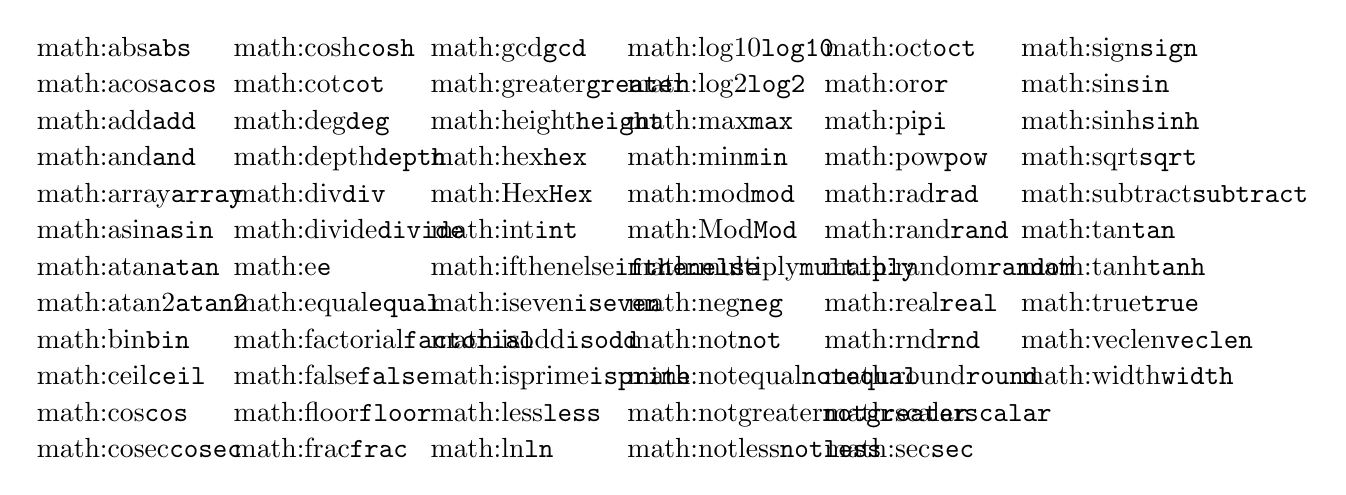
\begin{tikzpicture}
\foreach \f [count=\i from 0] in
{abs,acos,add,and,array,asin,atan,atan2,bin,ceil,cos,
 cosec,cosh,cot,deg,depth,div,divide,e,equal,factorial, false,
 floor,frac,gcd,greater,height,hex,Hex,int,ifthenelse,iseven,isodd,isprime,
 less,ln,log10,log2,max,min,mod,Mod,multiply,
 neg,not,notequal,notgreater,notless,
 oct,or,pi,pow,rad,rand,random,real,rnd,round,
 scalar,sec,sign,sin,sinh,sqrt,subtract,tan,tanh,true, veclen,width}
\node [anchor=base west] at ({int(\i/12)*2.5cm},{-mod(\i,12)*1.1*\baselineskip}) {\mathlink{\f}};
\end{tikzpicture}
\bigskip

Each function has a \pgfname{} command associated with it (which is also shown
with the function below). In general, the command is simply the name of the
function prefixed with |\pgfmath|, for example, |\pgfmathadd|, but there are
some notable exceptions.


\subsubsection{Basic arithmetic functions}
\label{pgfmath-functions-basic}

\begin{math-function}{add(\mvar{x},\mvar{y})}
\mathcommand
    Adds $x$ and $y$.
    %
\begin{codeexample}[]
\pgfmathparse{add(75,6)} \pgfmathresult
\end{codeexample}
    %
\end{math-function}

\begin{math-function}{subtract(\mvar{x},\mvar{y})}
\mathcommand
    Subtract $x$ from $y$.
    %
\begin{codeexample}[]
\pgfmathparse{subtract(75,6)} \pgfmathresult
\end{codeexample}
    %
\end{math-function}

\begin{math-function}{neg(\mvar{x})}
\mathcommand
    This returns $-\mvar{x}$.
    %
\begin{codeexample}[]
\pgfmathparse{neg(50)} \pgfmathresult
\end{codeexample}
    %
\end{math-function}

\begin{math-function}{multiply(\mvar{x},\mvar{y})}
\mathcommand
    Multiply $x$ by $y$.
    %
\begin{codeexample}[]
\pgfmathparse{multiply(75,6)} \pgfmathresult
\end{codeexample}
    %
\end{math-function}

\begin{math-function}{divide(\mvar{x},\mvar{y})}
\mathcommand
    Divide $x$ by $y$.
    %
\begin{codeexample}[]
\pgfmathparse{divide(75,6)} \pgfmathresult
\end{codeexample}
    %
\end{math-function}

\begin{math-function}{div(\mvar{x},\mvar{y})}
\mathcommand
    Divide $x$ by $y$ and return the integer part of the result.
    %
\begin{codeexample}[]
\pgfmathparse{div(75,9)} \pgfmathresult
\end{codeexample}
    %
\end{math-function}

\begin{math-function}{factorial(\mvar{x})}
\mathcommand
    Return \mvar{x}!.
    %
\begin{codeexample}[]
\pgfmathparse{factorial(5)} \pgfmathresult
\end{codeexample}
    %
\end{math-function}

\begin{math-function}{sqrt(\mvar{x})}
\mathcommand
    Calculates $\sqrt{\textrm{\mvar{x}}}$.
    %
\begin{codeexample}[]
\pgfmathparse{sqrt(10)} \pgfmathresult
\end{codeexample}

\begin{codeexample}[]
\pgfmathparse{sqrt(8765.432)} \pgfmathresult
\end{codeexample}
    %
\end{math-function}

\begin{math-function}{pow(\mvar{x},\mvar{y})}
\mathcommand
    Raises \mvar{x} to the power \mvar{y}. For greatest accuracy, \mvar{y}
    should be an integer. If \mvar{y} is not an integer, the actual calculation
    will be an approximation of $e^{y \ln(x)}$.
    %
\begin{codeexample}[]
\pgfmathparse{pow(2,7)} \pgfmathresult
\end{codeexample}
    %
\end{math-function}

\begin{math-function}{e}
\mathcommand
    Returns the value 2.718281828.
    %
{
\catcode`\^=7
\begin{codeexample}[]
\pgfmathparse{(e^2-e^-2)/2} \pgfmathresult
\end{codeexample}
}
\end{math-function}

\begin{math-function}{exp(\mvar{x})}
\mathcommand
{ \catcode`\^=7

    Maclaurin series for $e^x$.
}
\begin{codeexample}[]
\pgfmathparse{exp(1)} \pgfmathresult
\end{codeexample}

\begin{codeexample}[]
\pgfmathparse{exp(2.34)} \pgfmathresult
\end{codeexample}
    %
\end{math-function}

\begin{math-function}{ln(\mvar{x})}
\mathcommand
{ \catcode`\^=7
    An approximation for $\ln(\textrm{\mvar{x}})$. This uses an algorithm of
    Rouben Rostamian, and coefficients suggested by Alain Matthes.
}
\begin{codeexample}[]
\pgfmathparse{ln(10)} \pgfmathresult
\end{codeexample}

\begin{codeexample}[]
\pgfmathparse{ln(exp(5))} \pgfmathresult
\end{codeexample}
    %
\end{math-function}

\begin{math-function}{log10(\mvar{x})}
\mathcommand[logten(\mvar{x})]
    An approximation for $\log_{10}(\textrm{\mvar{x}})$.
    %
\begin{codeexample}[]
\pgfmathparse{log10(100)} \pgfmathresult
\end{codeexample}
    %
\end{math-function}

\begin{math-function}{log2(\mvar{x})}
\mathcommand[logtwo(\mvar{x})]
    An approximation for $\log_2(\textrm{\mvar{x}})$.
    %
\begin{codeexample}[]
\pgfmathparse{log2(128)} \pgfmathresult
\end{codeexample}
    %
\end{math-function}

\begin{math-function}{abs(\mvar{x})}
\mathcommand
    Evaluates the absolute value of $x$.
    %
\begin{codeexample}[]
\pgfmathparse{abs(-5)} \pgfmathresult
\end{codeexample}

\begin{codeexample}[]
\pgfmathparse{-abs(4*-3)} \pgfmathresult
\end{codeexample}
    %
\end{math-function}

\begin{math-function}{mod(\mvar{x},\mvar{y})}
\mathcommand
    This evaluates \mvar{x} modulo \mvar{y}, using truncated division. The sign
    of the result is the same as the sign of
    $\frac{\textrm{\mvar{x}}}{\textrm{\mvar{y}}}$.
    %
\begin{codeexample}[]
\pgfmathparse{mod(20,6)} \pgfmathresult
\end{codeexample}

\begin{codeexample}[]
\pgfmathparse{mod(-100,30)} \pgfmathresult
\end{codeexample}
    %
\end{math-function}

\begin{math-function}{Mod(\mvar{x},\mvar{y})}
\mathcommand
    This evaluates \mvar{x} modulo \mvar{y}, using floored division. The sign
    of the result is never negative.
    %
\begin{codeexample}[]
\pgfmathparse{Mod(-100,30)} \pgfmathresult
\end{codeexample}
    %
\end{math-function}

\begin{math-function}{sign(\mvar{x})}
\mathcommand
    Returns the sign of $x$.
    %
\begin{codeexample}[]
\pgfmathparse{sign(-5)} \pgfmathresult
\end{codeexample}

\begin{codeexample}[]
\pgfmathparse{sign(0)} \pgfmathresult
\end{codeexample}

\begin{codeexample}[]
\pgfmathparse{sign(5)} \pgfmathresult
\end{codeexample}
    %
\end{math-function}


\subsubsection{Rounding functions}
\label{pgfmath-functions-rounding}

\begin{math-function}{round(\mvar{x})}
\mathcommand
    Rounds \mvar{x} to the nearest integer. It uses ``asymmetric half-up''
    rounding. So |1.5| is rounded to |2|, but |-1.5| is rounded to |-2|
    (\emph{not} |-1|).
    %
\begin{codeexample}[]
\pgfmathparse{round(32.5/17)} \pgfmathresult
\end{codeexample}

\begin{codeexample}[]
\pgfmathparse{round(398/12)} \pgfmathresult
\end{codeexample}
    %
\end{math-function}

\begin{math-function}{floor(\mvar{x})}
\mathcommand
    Rounds \mvar{x} down to the nearest integer.
    %
\begin{codeexample}[]
\pgfmathparse{floor(32.5/17)} \pgfmathresult
\end{codeexample}

\begin{codeexample}[]
\pgfmathparse{floor(398/12)} \pgfmathresult
\end{codeexample}

\begin{codeexample}[]
\pgfmathparse{floor(-398/12)} \pgfmathresult
\end{codeexample}
    %
\end{math-function}

\begin{math-function}{ceil(\mvar{x})}
\mathcommand
    Rounds \mvar{x} up to the nearest integer.
    %
\begin{codeexample}[]
\pgfmathparse{ceil(32.5/17)} \pgfmathresult
\end{codeexample}

\begin{codeexample}[]
\pgfmathparse{ceil(398/12)} \pgfmathresult
\end{codeexample}

\begin{codeexample}[]
\pgfmathparse{ceil(-398/12)} \pgfmathresult
\end{codeexample}
    %
\end{math-function}

\begin{math-function}{int(\mvar{x})}
\mathcommand
    Returns the integer part of \mvar{x}.
    %
\begin{codeexample}[]
\pgfmathparse{int(32.5/17)} \pgfmathresult
\end{codeexample}
    %
\end{math-function}

\begin{math-function}{frac(\mvar{x})}
\mathcommand
    Returns the fractional part of \mvar{x}.
    %
\begin{codeexample}[]
\pgfmathparse{frac(32.5/17)} \pgfmathresult
\end{codeexample}
    %
\end{math-function}

\begin{math-function}{real(\mvar{x})}
\mathcommand
    Ensures \mvar{x} contains a decimal point.
    %
\begin{codeexample}[]
\pgfmathparse{real(4)} \pgfmathresult
\end{codeexample}
    %
\end{math-function}


\subsubsection{Integer arithmetics functions}
\label{pgfmath-functions-integerarithmetics}

\begin{math-function}{gcd(\mvar{x},\mvar{y})}
\mathcommand
    Computes the greatest common divider of \mvar{x} and \mvar{y}.
    %
\begin{codeexample}[]
\pgfmathparse{gcd(42,56)} \pgfmathresult
\end{codeexample}
    %
\end{math-function}

\begin{math-function}{isodd(\mvar{x})}
\mathcommand
    Returns |1| if the integer part of \mvar{x} is odd. Otherwise, returns |0|.
    %
\begin{codeexample}[]
\pgfmathparse{isodd(2)} \pgfmathresult,
\pgfmathparse{isodd(3)} \pgfmathresult
\end{codeexample}
    %
\end{math-function}

\begin{math-function}{iseven(\mvar{x})}
\mathcommand
    Returns |1| if the integer part of \mvar{x} is even. Otherwise, returns |0|.
    %
\begin{codeexample}[]
\pgfmathparse{iseven(2)} \pgfmathresult,
\pgfmathparse{iseven(3)} \pgfmathresult
\end{codeexample}
    %
\end{math-function}

\begin{math-function}{isprime(\mvar{x})}
\mathcommand
    Returns |1| if the integer part of \mvar{x} is prime. Otherwise, returns |0|.
    %
\begin{codeexample}[]
\pgfmathparse{isprime(1)} \pgfmathresult,
\pgfmathparse{isprime(2)} \pgfmathresult,
\pgfmathparse{isprime(31)} \pgfmathresult,
\pgfmathparse{isprime(64)} \pgfmathresult
\end{codeexample}
    %
\end{math-function}


\subsubsection{Trigonometric functions}
\label{pgfmath-functions-trigonometric}

\begin{math-function}{pi}
\mathcommand
    Returns the value $\pi=3.141592654$.
    %
\begin{codeexample}[]
\pgfmathparse{pi} \pgfmathresult
\end{codeexample}

\begin{codeexample}[]
\pgfmathparse{pi r} \pgfmathresult
\end{codeexample}
    %
\end{math-function}

\begin{math-function}{rad(\mvar{x})}
\mathcommand
    Convert \mvar{x} to radians. \mvar{x} is assumed to be in degrees.
    %
\begin{codeexample}[]
\pgfmathparse{rad(90)} \pgfmathresult
\end{codeexample}
    %
\end{math-function}

\begin{math-function}{deg(\mvar{x})}
\mathcommand
    Convert \mvar{x} to degrees. \mvar{x} is assumed to be in radians.
    %
\begin{codeexample}[]
\pgfmathparse{deg(3*pi/2)} \pgfmathresult
\end{codeexample}
    %
\end{math-function}

\begin{math-function}{sin(\mvar{x})}
\mathcommand
    %
    Sine of \mvar{x}. By employing the |r| operator, \mvar{x} can be in
    radians.
    %
\begin{codeexample}[]
\pgfmathparse{sin(60)} \pgfmathresult
\end{codeexample}

\begin{codeexample}[]
\pgfmathparse{sin(pi/3 r)} \pgfmathresult
\end{codeexample}
    %
\end{math-function}

\begin{math-function}{cos(\mvar{x})}
\mathcommand
    Cosine of \mvar{x}. By employing the |r| operator, \mvar{x} can be in
    radians.
    %
\begin{codeexample}[]
\pgfmathparse{cos(60)} \pgfmathresult
\end{codeexample}

\begin{codeexample}[]
\pgfmathparse{cos(pi/3 r)} \pgfmathresult
\end{codeexample}
    %
\end{math-function}

\begin{math-function}{tan(\mvar{x})}
\mathcommand
    Tangent of \mvar{x}. By employing the |r| operator, \mvar{x} can be in
    radians.
    %
\begin{codeexample}[]
\pgfmathparse{tan(45)} \pgfmathresult
\end{codeexample}

\begin{codeexample}[]
\pgfmathparse{tan(2*pi/8 r)} \pgfmathresult
\end{codeexample}
    %
\end{math-function}

\begin{math-function}{sec(\mvar{x})}
\mathcommand
    Secant of \mvar{x}. By employing the |r| operator, \mvar{x} can be in
    radians.
    %
\begin{codeexample}[]
\pgfmathparse{sec(45)} \pgfmathresult
\end{codeexample}
    %
\end{math-function}

\begin{math-function}{cosec(\mvar{x})}
\mathcommand
    Cosecant of \mvar{x}. By employing the |r| operator, \mvar{x} can be in
    radians.
    %
\begin{codeexample}[]
\pgfmathparse{cosec(30)} \pgfmathresult
\end{codeexample}
    %
\end{math-function}

\begin{math-function}{cot(\mvar{x})}
\mathcommand
    Cotangent of \mvar{x}. By employing the |r| operator, \mvar{x} can be in
    radians.
    %
\begin{codeexample}[]
\pgfmathparse{cot(15)} \pgfmathresult
\end{codeexample}
    %
\end{math-function}

\begin{math-function}{asin(\mvar{x})}
\mathcommand
    Arcsine of \mvar{x}. The result is in degrees and in the range $\pm90^\circ$.
    %
\begin{codeexample}[]
\pgfmathparse{asin(0.7071)} \pgfmathresult
\end{codeexample}
    %
\end{math-function}

\begin{math-function}{acos(\mvar{x})}
\mathcommand
    Arccosine of \mvar{x} in degrees. The result is in the range $[0^\circ,180^\circ]$.
    %
\begin{codeexample}[]
\pgfmathparse{acos(0.5)} \pgfmathresult
\end{codeexample}
    %
\end{math-function}

\begin{math-function}{atan(\mvar{x})}
\mathcommand
    Arctangent of $x$ in degrees.
    %
\begin{codeexample}[]
\pgfmathparse{atan(1)} \pgfmathresult
\end{codeexample}
    %
\end{math-function}

\begin{math-function}{atan2(\mvar{y},\mvar{x})}
\mathcommand[atantwo(\mvar{y},\mvar{x})]
    Arctangent of $y\div x$ in degrees. This also takes into account the
    quadrants.
    %
\begin{codeexample}[]
\pgfmathparse{atan2(-4,3)} \pgfmathresult
\end{codeexample}
    %
\end{math-function}

\begin{key}{/pgf/trig format=\mchoice{deg,rad} (initially deg)}
    Allows to define whether trigonometric math functions (i.e.\ all in this
    subsection) operate with degrees or with radians.
    %
\begin{codeexample}[]
\pgfmathparse{cos(45)} \pgfmathresult
\end{codeexample}
\begin{codeexample}[]
\pgfkeys{/pgf/trig format=rad}
\pgfmathparse{cos(pi/2)} \pgfmathresult
\end{codeexample}

    The initial configuration |trig format=deg| is the base of \pgfname: almost
    all of it is based on degrees.

    Specifying |trig format=rad| is most useful for data visualization where
    the angles are typically given in radians. However, it is applied to all
    trigonometric functions for which the option applies, including any drawing
    instructions which operate on angles.
    %
\begin{codeexample}[]
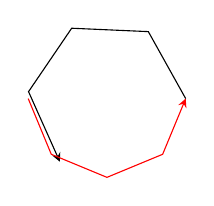
\begin{tikzpicture}
    \draw[-stealth]
        (0:1) -- (45:1) -- (90:1) -- (135:1) -- (180:1);

    \draw[-stealth,trig format=rad,red]
        (pi:1) -- (5/4*pi:1) -- (6/4*pi:1) -- (7/4*pi:1) -- (2*pi:1);
\end{tikzpicture}
\end{codeexample}

    \paragraph{Warning:}
    At the time of this writing, this feature is ``experimental''. Please
    handle it with care: there may be path instructions or libraries in
    \pgfname\ which rely on |trig format=deg|. The intended usage of
    |trig format=rad| is for local scopes -- and as option for data
    visualization.
\end{key}


\subsubsection{Comparison and logical functions}
\label{pgfmath-functions-comparison}

\begin{math-function}{equal(\mvar{x},\mvar{y})}
\mathcommand
    This returns |1| if $\mvar{x}=\mvar{y}$ and |0| otherwise.
    %
\begin{codeexample}[]
\pgfmathparse{equal(20,20)} \pgfmathresult
\end{codeexample}
    %
\end{math-function}

\begin{math-function}{greater(\mvar{x},\mvar{y})}
\mathcommand
    This returns |1| if $\mvar{x}>\mvar{y}$ and |0| otherwise.
    %
\begin{codeexample}[]
\pgfmathparse{greater(20,25)} \pgfmathresult
\end{codeexample}
    %
\end{math-function}

\begin{math-function}{less(\mvar{x},\mvar{y})}
\mathcommand
    This returns |1| if $\mvar{x}<\mvar{y}$ and |0| otherwise.
    %
\begin{codeexample}[]
\pgfmathparse{greater(20,25)} \pgfmathresult
\end{codeexample}
    %
\end{math-function}

\begin{math-function}{notequal(\mvar{x},\mvar{y})}
\mathcommand
    This returns |0| if $\mvar{x}=\mvar{y}$ and |1| otherwise.
    %
\begin{codeexample}[]
\pgfmathparse{notequal(20,25)} \pgfmathresult
\end{codeexample}
    %
\end{math-function}

\begin{math-function}{notgreater(\mvar{x},\mvar{y})}
\mathcommand
    This returns |1| if $\mvar{x}\leq\mvar{y}$ and |0| otherwise.
    %
\begin{codeexample}[]
\pgfmathparse{notgreater(20,25)} \pgfmathresult
\end{codeexample}
    %
\end{math-function}

\begin{math-function}{notless(\mvar{x},\mvar{y})}
\mathcommand
    This returns |1| if $\mvar{x}\geq\mvar{y}$ and |0| otherwise.
    %
\begin{codeexample}[]
\pgfmathparse{notless(20,25)} \pgfmathresult
\end{codeexample}
    %
\end{math-function}

\begin{math-function}{and(\mvar{x},\mvar{y})}
\mathcommand
    This returns |1| if \mvar{x} and \mvar{y} both evaluate to non-zero values.
    Otherwise |0| is returned.
    %
\begin{codeexample}[]
\pgfmathparse{and(5>4,6>7)} \pgfmathresult
\end{codeexample}
    %
\end{math-function}

\begin{math-function}{or(\mvar{x},\mvar{y})}
\mathcommand
    This returns |1| if either \mvar{x} or \mvar{y} evaluate to non-zero
    values. Otherwise |0| is returned.
    %
\begin{codeexample}[]
\pgfmathparse{or(5>4,6>7)} \pgfmathresult
\end{codeexample}
    %
\end{math-function}

\begin{math-function}{not(\mvar{x})}
\mathcommand
    This returns |1| if $\mvar{x}=0$, otherwise |0|.
    %
\begin{codeexample}[]
\pgfmathparse{not(true)} \pgfmathresult
\end{codeexample}
    %
\end{math-function}

\begin{math-function}{ifthenelse(\mvar{x},\mvar{y},\mvar{z})}
\mathcommand
    This returns \mvar{y} if \mvar{x} evaluates to some non-zero value,
    otherwise \mvar{z} is returned.
    %
\begin{codeexample}[]
\pgfmathparse{ifthenelse(5==4,"yes","no")} \pgfmathresult
\end{codeexample}
    %
\end{math-function}

\begin{math-function}{true}
\mathcommand
    This evaluates to |1|.
    %
\begin{codeexample}[]
\pgfmathparse{true ? "yes" : "no"} \pgfmathresult
\end{codeexample}
    %
\end{math-function}

\begin{math-function}{false}
\mathcommand
    This evaluates to |0|.
    %
\begin{codeexample}[]
\pgfmathparse{false ? "yes" : "no"} \pgfmathresult
\end{codeexample}
    %
\end{math-function}


\subsubsection{Pseudo-random functions}
\label{pgfmath-functions-random}

\begin{math-function}{rnd}
\mathcommand
    Generates a pseudo-random number between $0$ and $1$ with a uniform
    distribution.
    %
\begin{codeexample}[pre={\pgfmathsetseed{1}}]
\foreach \x in {1,...,10}{\pgfmathparse{rnd}\pgfmathresult, }
\end{codeexample}
    %
\end{math-function}

\begin{math-function}{rand}
\mathcommand
    Generates a pseudo-random number between $-1$ and $1$ with a uniform
    distribution.
    %
\begin{codeexample}[pre={\pgfmathsetseed{1}}]
\foreach \x in {1,...,10}{\pgfmathparse{rand}\pgfmathresult, }
\end{codeexample}
    %
\end{math-function}

\begin{math-function}{random(\opt{\mvar{x},\mvar{y}})}
\mathcommand
    This function takes zero, one or two arguments. If there are zero
    arguments, a uniform random number between $0$ and $1$ is generated. If
    there is one argument \mvar{x}, a random integer between $1$ and \mvar{x}
    is generated. Finally, if there are two arguments, a random integer between
    \mvar{x} and \mvar{y} is generated. If there are no arguments, the
    \pgfname{} command should be called as follows: |\pgfmathrandom{}|.
    %
\begin{codeexample}[pre={\pgfmathsetseed{1}}]
\foreach \x in {1,...,10}{\pgfmathparse{random()}\pgfmathresult, }
\end{codeexample}

\begin{codeexample}[pre={\pgfmathsetseed{1}}]
\foreach \x in {1,...,10}{\pgfmathparse{random(100)}\pgfmathresult, }
\end{codeexample}

\begin{codeexample}[pre={\pgfmathsetseed{1}}]
\foreach \x in {1,...,10}{\pgfmathparse{random(232,762)}\pgfmathresult, }
\end{codeexample}
    %
\end{math-function}


\subsubsection{Base conversion functions}
\label{pgfmath-functions-base}

\begin{math-function}{hex(\mvar{x})}
\mathcommand
    Convert \mvar{x}{} (assumed to be an integer in base 10) to a hexadecimal
    representation, using lower case alphabetic digits. No further calculation
    will be possible with the result.
    %
\begin{codeexample}[]
\pgfmathparse{hex(65535)} \pgfmathresult
\end{codeexample}
    %
\end{math-function}

\begin{math-function}{Hex(\mvar{x})}
\mathcommand
    Convert \mvar{x}{} (assumed to be an integer in base 10) to a hexadecimal
    representation, using upper case alphabetic digits. No further calculation
    will be possible with the result.
    %
\begin{codeexample}[]
\pgfmathparse{Hex(65535)} \pgfmathresult
\end{codeexample}
    %
\end{math-function}

\begin{math-function}{oct(\mvar{x})}
\mathcommand
    Convert \mvar{x}{} (assumed to be an integer in base 10) to an octal
    representation. No further calculation should be attempted with the result,
    as the parser can only process numbers converted to base 10.
    %
\begin{codeexample}[]
\pgfmathparse{oct(63)} \pgfmathresult
\end{codeexample}
    %
\end{math-function}

\begin{math-function}{bin(\mvar{x})}
\mathcommand
    Convert \mvar{x}{} (assumed to be an integer in base 10) to a binary
    representation. No further calculation should be attempted with the result,
    as the parser can only process numbers converted to base 10.
    %
\begin{codeexample}[]
\pgfmathparse{bin(185)} \pgfmathresult
\end{codeexample}
    %
\end{math-function}


\subsubsection{Miscellaneous functions}
\label{pgfmath-functions-misc}

\begin{math-function}{min(\mvar{x$_1$},\mvar{x$_2$},\ldots,\mvar{x$_n$})}
\mathcommand[min({\mvar{x$_1$},\mvar{x$_2$},\ldots},{\ldots,\mvar{x$_{n-1}$},\mvar{x$_n$}})]
    Return the minimum value from \mvar{x$_1$}\ldots\mvar{x$_n$}. For
    historical reasons, the command |\pgfmathmin| takes two arguments, but each
    of these can contain an arbitrary number of comma separated values.
    %
\begin{codeexample}[]
\pgfmathparse{min(3,4,-2,250,-8,100)} \pgfmathresult
\end{codeexample}
    %
\end{math-function}

\begin{math-function}{max(\mvar{x$_1$},\mvar{x$_2$},\ldots,\mvar{x$_n$})}
\mathcommand[max({\mvar{x$_1$},\mvar{x$_2$},\ldots},{\ldots,\mvar{x$_{n-1}$},\mvar{x$_n$}})]
    Return the maximum value from \mvar{x$_1$}\ldots\mvar{x$_n$}. Again, for
    historical reasons, the command |\pgfmathmax| takes two arguments, but each
    of these can contain an arbitrary number of comma separated values.
    %
\begin{codeexample}[]
\pgfmathparse{max(3,4,-2,250,-8,100)} \pgfmathresult
\end{codeexample}
    %
\end{math-function}

\begin{math-function}{veclen(\mvar{x},\mvar{y})}
\mathcommand
    Calculates $\sqrt{\left(\textrm{\mvar{x}}^2+\textrm{\mvar{y}}^2\right)}$.
    This uses a polynomial approximation, based on ideas of Rouben Rostamian
    %
\begin{codeexample}[]
\pgfmathparse{veclen(12,5)} \pgfmathresult
\end{codeexample}
    %
\end{math-function}

\begin{math-function}{array(\mvar{x},\mvar{y})}
\mathcommand
    This accesses the array \mvar{x} at the index \mvar{y}. The array must
    begin and end with braces (e.g., |{1,2,3,4}|) and array indexing starts at
    |0|.
    %
\begin{codeexample}[]
\pgfmathparse{array({9,13,17,21},2)} \pgfmathresult
\end{codeexample}
    %
\end{math-function}

The following hyperbolic functions were adapted from code suggested by Martin
Heller:

\begin{math-function}{sinh(\mvar{x})}
\mathcommand
    The hyperbolic sine of \mvar{x}
    %
\begin{codeexample}[]
\pgfmathparse{sinh(0.5)} \pgfmathresult
\end{codeexample}
    %
\end{math-function}

\begin{math-function}{cosh(\mvar{x})}
\mathcommand
    The hyperbolic cosine of \mvar{x}
    %
\begin{codeexample}[]
\pgfmathparse{cosh(0.5)} \pgfmathresult
\end{codeexample}
    %
\end{math-function}

\begin{math-function}{tanh(\mvar{x})}
\mathcommand
    The hyperbolic tangent of \mvar{x}
    %

\begin{codeexample}[]
\pgfmathparse{tanh(0.5)} \pgfmathresult
\end{codeexample}
    %
\end{math-function}

\begin{math-function}{width("\mvar{x}")}
\mathcommand
    Return the width of a \TeX{} (horizontal) box containing \mvar{x}. The
    quote characters are necessary to prevent \mvar{x}{} from being parsed. It
    is important to remember that any expression is expanded with |\edef|
    before being parsed, so any macros (e.g., font commands like |\tt| or
    |\Huge|) will need to be ``protected'' (e.g., |\noexpand\Huge| is usually
    sufficient).
    %
\begin{codeexample}[]
\pgfmathparse{width("Some Lovely Text")} \pgfmathresult
\end{codeexample}

    Note that results of this method are provided in points.
\end{math-function}

\begin{math-function}{height("\mvar{x}")}
\mathcommand
    Return the height of a box containing \mvar{x}.
    %
\begin{codeexample}[]
\pgfmathparse{height("Some Lovely Text")} \pgfmathresult
\end{codeexample}
    %
\end{math-function}

\begin{math-function}{depth("\mvar{x}")}
\mathcommand
    Returns the depth of a box containing \mvar{x}.
    %
\begin{codeexample}[]
\pgfmathparse{depth("Some Lovely Text")} \pgfmathresult
\end{codeexample}
    %
\end{math-function}
